\documentclass{article}

\usepackage{tikz}
\usepackage{pdfpages}
\usepackage{parskip}
\usepackage{amsmath}
\usepackage[margin=.6in]{geometry}

\begin{document}
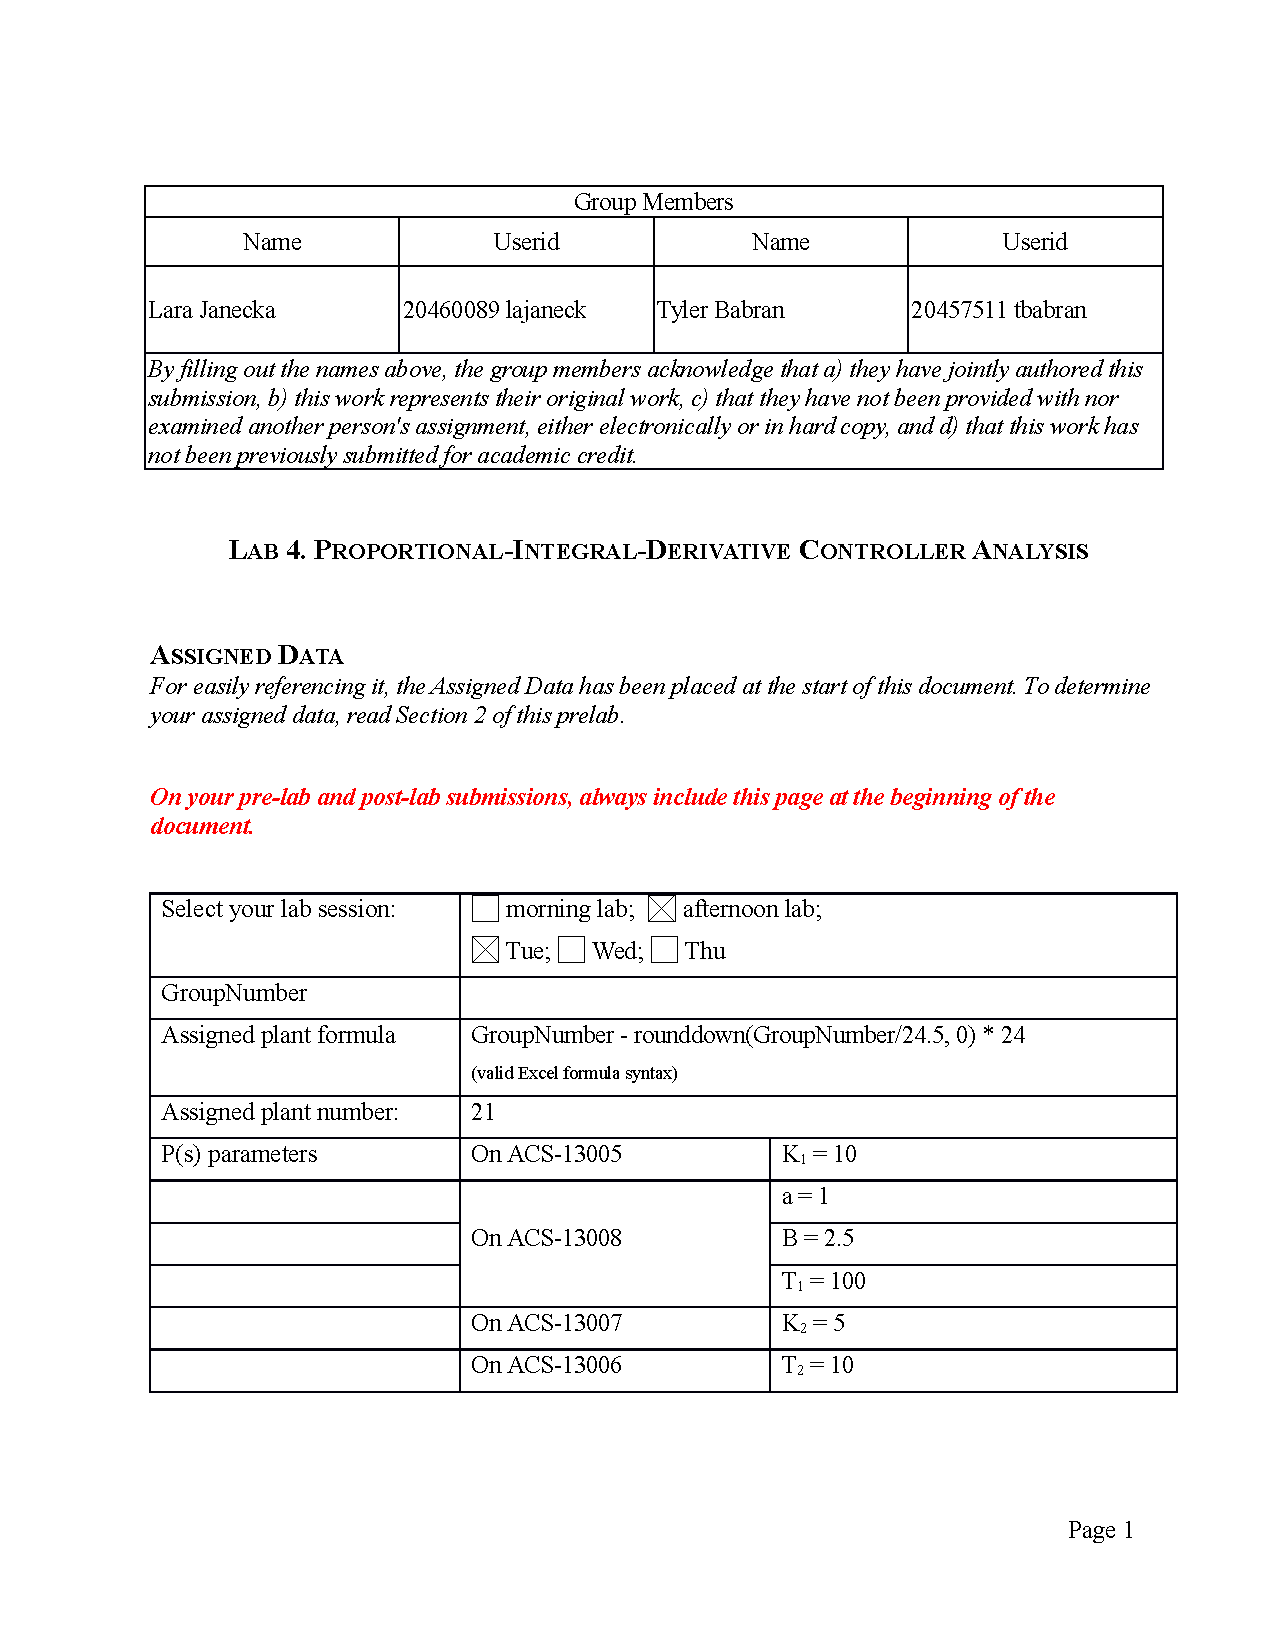
\includepdf[pages={1}]{page1.pdf}

\section*{a)} % (fold)
\label{sec:a_}
\begin{align*}
    \text{M(S)} &= \frac{\frac{K_1bT_1}{s(s+aT_1)}}{1+\frac{K_1bT_1}{s(s+aT_1)}}\\
                &= \frac{K_1bT_1}{s(s+aT_1)} \times \frac{s(s+aT_1)}{{s(s+aT_1)} + K_1bT_1}\\
                &= \frac{K_1bT_1}{{s(s+aT_1)} + K_1bT_1}\\
                &= \frac{K_1bT_1}{s^2 + saT_1 + K_1bT_1}\\
\end{align*}


\begin{align*}
    \text{N(S)} &= \frac{\frac{K_2T_2}{s}}{1 + \frac{K_2T_2}{s}}\\
                &= \frac{K_2T_2}{s + K_2T_2}\\
                &= \frac{1}{\frac{s}{K_2T_2} + 1}
\end{align*}


\begin{align*}
    \text{P(S)} &= \text{M(S)} \times \text{N(S)}\\
                &= \frac{K_1bT_1}{s^2 + saT_1 + K_1bT_1} \times \frac{K_2T_2}{s + K_2T_2}\\
                &= \frac{bK_1T_1K_2T_2}{(s + K_2T_2)(s^2 + saT_1 + K_1bT_1)}\\
\end{align*}
% section a_ (end)

\section*{b)} % (fold)
\label{sec:b_}
\begin{align*}
    \text{H(S)} &=  \frac{K_p \times\text{P(S)}}{1 + K_p\text{P(S)}}\\
                &= \frac{K_pbK_1T_1K_2T_2}{(s + K_2T_2)(s^2 + saT_1 + K_1bT_1) + 2bK_1T_1K_2T_2}\\
                &= \frac{K_pbK_1T_1K_2T_2}{s^3 + (aT_1 + K_2T_2)s^2 + (K_1bT_1 + K_2T_2aT_1)s + 2K_2T_2K_1bT_1}\\
                &= \frac{125000}{s^3 + (150)s^2 + (7500)s + 250000}\\
\end{align*}

\begin{table}[!htbp]
\centering
    \begin{tabular}{|c|c|c|}
        \hline
        \textbf{Output Parameter} & \textbf{Symbol} & \textbf{Value} \\
        \hline
        Magnitude of first peak & $M_p$ & 0.14\\
        \hline
        Time to First Peak & $T_p$ & 0.084\\
        \hline
        Settling Time (2\%) & $T_s$ & 0.168\\
        \hline
        Steady-state & $y_ss$ & 0.1\\
        \hline
    \end{tabular}
    \caption{step-response characteristics}
\end{table}

\begin{figure}[!htbp]
\centering
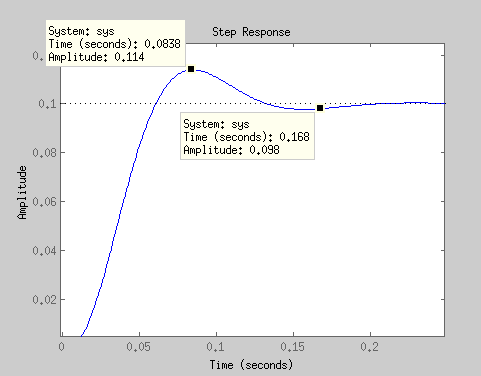
\includegraphics[width=6.5in]{prelab-2vStepResponse.png}
\caption{Step response of system}
\end{figure}

% section b_ (end)

\section*{c)} % (fold)
\label{sec:c_}
Since the system is strictly proper its stability is determined by the presence of roots in the positive real area.
\begin{align*}
    \text{H(S)} &= \frac{125000}{s^3 + (150)s^2 + (7500)s + 125000(1+K_p)}\\
    \text{Q(S)} &= s^3 + (150)s^2 + (7500)s + 250000\\
    a_3 &= 1\\
    a_2 &= 150\\
    a_1 &= 7500\\
    a_0 &= 125000(1+K_p)\\
    b_1 &= \frac{-1}{150} \times
    \begin{vmatrix}
    1 & 7500  \\
    150 & 125000(1+K_p) \notag
    \end{vmatrix}\\
    &= 7500 - 833.33(1+K_p)\\
    c_0 &=  \frac{-1}{7500 - 833.33(1+K_p)} \times
    \begin{vmatrix}
    150 & 125000(1+K_p)  \\
    7500 - 833.33(1+K_p) & 0 \notag
    \end{vmatrix}\\
    &= 125000(1+K_p)\\
\end{align*}

\begin{table}[!htbp]
\centering
    \begin{tabular}{c|c c}
    3 & 1 & 7500\\
    2 & 150 & 250000\\
    1 & $7500 - 833.33(1+K_p)$ & 0\\
    0 & 250000 & 0\\
    \end{tabular}
\end{table}

This means that the system is stable where:
\begin{align*}
    7500 - 833.33(1+K_p) & > 0\\
    K_p > 8
\end{align*}






% section c_ (end)




\end{document}
